\subsection{Estrutura Organizacional}

\subsubsection{2. Estrutura Organizacional}

Hermathena = Ecossistema de Comunicação Científica

Laniakea  \rightarrow Governança
Virgo     \rightarrow Steering Committee

Magellan  \rightarrow Tecnologia
Via Láctea \rightarrow Educação
Andromeda \rightarrow Engajamento
Triangulum \rightarrow Conteúdo profundo

\begin{figure}[!htbp]
\centering
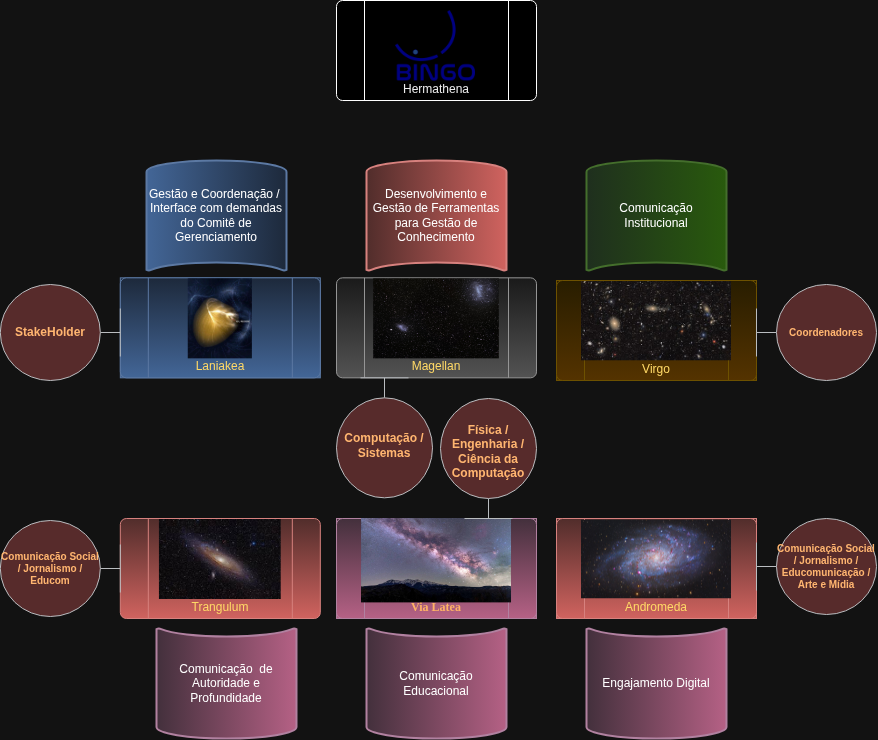
\includegraphics[width=1\linewidth]{files/nucleos-b9222e3152f6e2ffed5593f446132d20.png}
\end{figure}

\paragraph{2.1 Núcleos de Atuação}

O projeto está organizado em \textbf{núcleos}, cada um com funções específicas, complementares e afinidade de área definida.

\subparagraph{Núcleo 0: Laniakea}

Corresponde aos stakeholders do projeto. É constituído por representantes dos coordenadores do projeto juntamente com representantes do gerenciamento do projeto radiotelescópio BINGO e demais atores relevantes, a exemplo de financiadores.

\subparagraph{Núcleo 1: Magellan --- Ferramentas TIC}

Encarregado de promover um workflow para os demais projetos que garanta a qualidade das informações, sua temporalidade, reservas de direito, promoção de uma boa experiência para os usuários de todos os níveis.

\bigskip\noindent
\begin{tabular}{p{\dimexpr 0.500\linewidth-2\tabcolsep}p{\dimexpr 0.500\linewidth-2\tabcolsep}}
\toprule
Atributo & Descrição \\
\hline
\textbf{Afinidade de Área} & Ciência da Computação / Análise e Desenvolvimento de Sistemas \\
\textbf{Função} & Desenvolvimento de ferramentas tecnológicas \\
\textbf{Responsabilidades} & Criação e manutenção de sistemas; Automação de tarefas; Desenvolvimento de soluções; UI/UX \\
\textbf{Produtos} & Portal web, sistemas de automação, dashboards, chatbot, app mobile \\
\bottomrule
\end{tabular}

\bigskip

\subparagraph{Núcleo 2: Virgo --- Steering Committee}

Este é o local de troca de informações dos coordenadores de todos os projetos, pode começar com uma estrutura muito enxuta, mas assume cada vez mais relevância ao agregarmos parceiros de outras instituições

\bigskip\noindent
\begin{tabular}{p{\dimexpr 0.500\linewidth-2\tabcolsep}p{\dimexpr 0.500\linewidth-2\tabcolsep}}
\toprule
Atributo & Descrição \\
\hline
\textbf{Composição} & Membro designado do grupo de gerenciamento do BINGO (ouvinte); profissionais de comunicação convidados; 1 membro do projeto de cada instituição parceira \\
\textbf{Função} & Coordenação estratégica e governança \\
\textbf{Responsabilidades} & Definição de diretrizes estratégicas; Aprovação de grandes decisões; Interface com colaboração BINGO internacional; Supervisão de resultados \\
\bottomrule
\end{tabular}

\bigskip

\subparagraph{Núcleo 3: Via Láctea --- Comunicação Educacional}

\bigskip\noindent
\begin{tabular}{p{\dimexpr 0.500\linewidth-2\tabcolsep}p{\dimexpr 0.500\linewidth-2\tabcolsep}}
\toprule
Atributo & Descrição \\
\hline
\textbf{Afinidade de Área} & Física / Engenharia Elétrica \\
\textbf{Função} & Comunicação educacional \\
\textbf{Responsabilidades} & Produção de material educacional; Construção de equipamentos de demonstração; conteúdo para Portal web; elaboração de roteiros, manuais, planos de experiências... \\
\textbf{Produtos} & Portal web, biblioteca educacional, manuais, equipamentos de demonstração \\
\bottomrule
\end{tabular}

\bigskip

\subparagraph{Núcleo 4: Andromeda --- Comunicação de Engajamento}

\bigskip\noindent
\begin{tabular}{p{\dimexpr 0.500\linewidth-2\tabcolsep}p{\dimexpr 0.500\linewidth-2\tabcolsep}}
\toprule
Atributo & Descrição \\
\hline
\textbf{Afinidade de Área} & Comunicação Social / Educomunicação / Arte e Mídia / Jornalismo \\
\textbf{Função} & Comunicação de engajamento digital \\
\textbf{Responsabilidades} & Gestão de redes sociais (Instagram, Facebook, TikTok); Produção de conteúdo viral; Interação com comunidade online; Métricas de engajamento \\
\textbf{Produtos} & Feed Instagram, Facebook, Reels, TikToks, campanhas temáticas \\
\bottomrule
\end{tabular}

\bigskip

\subparagraph{Núcleo 5: Triangulum --- Comunicação de Profundidade}

\bigskip\noindent
\begin{tabular}{p{\dimexpr 0.500\linewidth-2\tabcolsep}p{\dimexpr 0.500\linewidth-2\tabcolsep}}
\toprule
Atributo & Descrição \\
\hline
\textbf{Afinidade de Área} & Comunicação Social / Educomunicação / Arte e Mídia / Jornalismo / Cinema \\
\textbf{Função} & Comunicação de profundidade e autoridade \\
\textbf{Responsabilidades} & Produção audiovisual longo; Canais de streaming; Entrevistas e debates; Documentários e séries \\
\textbf{Produtos} & Podcasts Spotify, vídeos YouTube, documentários, webinários, lives \\
\bottomrule
\end{tabular}

\bigskip

Do ponto de vista da aplicação do programa ao PROBEX/UFCG, o núcleo \textit{Virgo} representa a coordenação do programa e os núcleos \textit{Magellan}, \textit{Triangullum}, \textit{Via Lactea} e \textit{Andromeda} representam os projetos.

\paragraph{2.2 Estrutura das Equipes}

Cada núcleo operacional (Via Láctea, Andromeda, Triangulum, Magellan) possui:

\bigskip\noindent
\begin{tabular}{p{\dimexpr 0.333\linewidth-2\tabcolsep}p{\dimexpr 0.333\linewidth-2\tabcolsep}p{\dimexpr 0.333\linewidth-2\tabcolsep}}
\toprule
Função & Quantidade & Perfil \\
\hline
\textbf{Professor Orientador} & 1 & Docente da área de afinidade \\
\textbf{Professor Colaborador} & 1 & Docente de área complementar \\
\textbf{Bolsista PROBEX} & 1 & Graduação na área de afinidade \\
\textbf{Voluntários} & 5 & Graduação em áreas afins \\
\bottomrule
\end{tabular}

\bigskip

\textbf{Expansão:} Os núcleos podem se replicar em instituições parceiras, atingindo até \textbf{12 alunos + 4 docentes} por núcleo distribuídos.

\paragraph{2.3 Dinâmica de Trabalho}

\bigskip\noindent
\begin{tabular}{p{\dimexpr 0.250\linewidth-2\tabcolsep}p{\dimexpr 0.250\linewidth-2\tabcolsep}p{\dimexpr 0.250\linewidth-2\tabcolsep}p{\dimexpr 0.250\linewidth-2\tabcolsep}}
\toprule
Reunião & Frequência & Participantes & Modalidade \\
\hline
\textbf{Núcleo - Reunião de Produção} & Quinzenal & Membros do núcleo & Presencial \\
\textbf{Núcleo - Reunião de Acompanhamento} & Quinzenal & Membros do núcleo & Online \\
\textbf{Steering Committee (Virgo)} & Mensal & Coordenadores de núcleos & Online \\
\textbf{Laniakea} & Trimestral & Membros do comitê & Online \\
\bottomrule
\end{tabular}

\bigskip